\documentclass[11pt,a4paper]{article}
\usepackage[a4paper,margin=19mm,headheight=15pt]{geometry}
\usepackage{fontspec}
\setmainfont{Times New Roman}
\setsansfont{Arial}
\usepackage{microtype}
\usepackage{graphicx,booktabs,tabularx,array,pdflscape,float,enumitem}
\usepackage{xcolor,hyperref,fancyhdr,amsmath,amssymb}
\hypersetup{colorlinks=false,pdfborder={0 0 0},pdfauthor={Vu Hung Anh},pdftitle={Multimodal Search System for E-Commerce -- Assignment 06 V02}}
\definecolor{navy}{HTML}{17365D}
\definecolor{pale}{HTML}{E7F2FB}
\pagestyle{fancy}\fancyhf{}
\lhead{Information System Analysis and Design}
\rhead{Assignment 06 -- V02}
\cfoot{\thepage}
\setlength{\parindent}{0pt}
\setlength{\parskip}{5pt}
\renewcommand{\arraystretch}{1.12}
\newcolumntype{Y}{>{\raggedright\arraybackslash}X}
\newcommand{\code}[1]{\texttt{#1}}
\newcommand{\nextsection}[1]{\clearpage\section{#1}}
\setlist[itemize]{leftmargin=1.4em,itemsep=2pt,topsep=3pt}
\begin{document}

\begin{titlepage}
\centering
\vspace*{13mm}
{\Large POSTS AND TELECOMMUNICATIONS INSTITUTE OF TECHNOLOGY\par}
\vspace{4mm}
{\large Information System Analysis and Design\par}
\vspace{23mm}
{\Huge\bfseries MULTIMODAL SEARCH SYSTEM\par}
\vspace{4mm}
{\LARGE\bfseries FOR E-COMMERCE\par}
\vspace{8mm}
{\Large Assignment 06 -- UML Design and Python Prototype\par}
\vspace{20mm}
\begin{tabular}{rl}
Student: & Vu Hung Anh \\
Student ID: & B23DCDT022 \\
Submission date: & 7 October 2026 \\
Submission version: & V02
\end{tabular}
\vspace{18mm}
\begin{minipage}{0.87\linewidth}
\textbf{Abstract.} This report presents an e-commerce search prototype for text, voice, and product images. V02 adds package-text recognition with Apple Vision OCR to the existing Apple Vision image search. On 80 held-out alternate-view photos, this combined method improves exact-product top-1 results from 20 to 28, compared with the original Vision-only ranking. The report includes the UML design, implementation, demonstration, and evaluation method.
\end{minipage}
\vfill
{\small Source code, the editable Visual Paradigm project, and dataset are linked on the final page.\par}
\end{titlepage}

\section{Problem and requirements}
Online customers search for products in different ways: they may type a description, speak a query, or provide a product image. The system converts each input to a common query format, retrieves candidate products, ranks them, and displays the results. Customers can also look up their own orders.

The prototype connects requirements analysis, UML design, a three-layer architecture, and executable Python code. It has a short console example and a local browser interface. The browser can recognize microphone speech and pass its transcript to Python; typed transcripts remain available. Image search uses Apple's Vision framework through a local Swift process on macOS.

\begin{center}
\fcolorbox{navy}{pale}{\parbox{0.88\linewidth}{\centering Text, voice, or image $\longrightarrow$ common query $\longrightarrow$ candidate retrieval $\longrightarrow$ ranking $\longrightarrow$ results}}
\end{center}

\textbf{Primary actor:} Customer. A customer ID is supplied for order lookup; the repository checks ownership before returning an order.

\begin{table}[H]\small
\caption{Functional requirements and implementation evidence}
\begin{tabularx}{\linewidth}{@{}p{12mm}Y Y@{}}\toprule
ID & Requirement & Evidence \\ \midrule
FR01 & Search products using text keywords or a short sentence. & Text normalization, filters, and ranked results. \\
FR02 & Search by voice input. & Browser speech recognition creates a transcript; SpeechService sends it to text retrieval. \\
FR03 & Search by product image. & ImageService validates the photo; Apple Vision encodes it for ranking. \\
FR04 & Use one query format and separate retrieval from ranking. & QueryService, SearchService, and RankingService. \\
FR05 & View a product and search or view a customer-owned order. & Product lookup and customer-scoped OrderService. \\
FR06 & Demonstrate the input, processing, and result for each required mode. & Browser and console output, plus saved evaluation cases. \\
\bottomrule\end{tabularx}
\end{table}

\begin{table}[H]\small
\caption{Non-functional requirements}
\begin{tabularx}{\linewidth}{@{}p{12mm}Y@{}}\toprule
ID & Requirement and response \\ \midrule
NFR01 & Maintainability: the presentation calls services; repositories handle data access. \\
NFR02 & Reproducibility: sample data, setup steps, and evaluation outputs are included. \\
NFR03 & Explainability: ranked results show the component scores used by the prototype. \\
NFR04 & Robustness and privacy: invalid empty inputs are rejected; order lookup checks customer ownership. \\
\bottomrule\end{tabularx}
\end{table}

The system returns up to five ranked products with scores. A query with no eligible product returns no matches. An unknown order or an order belonging to another customer is not returned.

\nextsection{Use-case model}
\begin{figure}[H]\centering
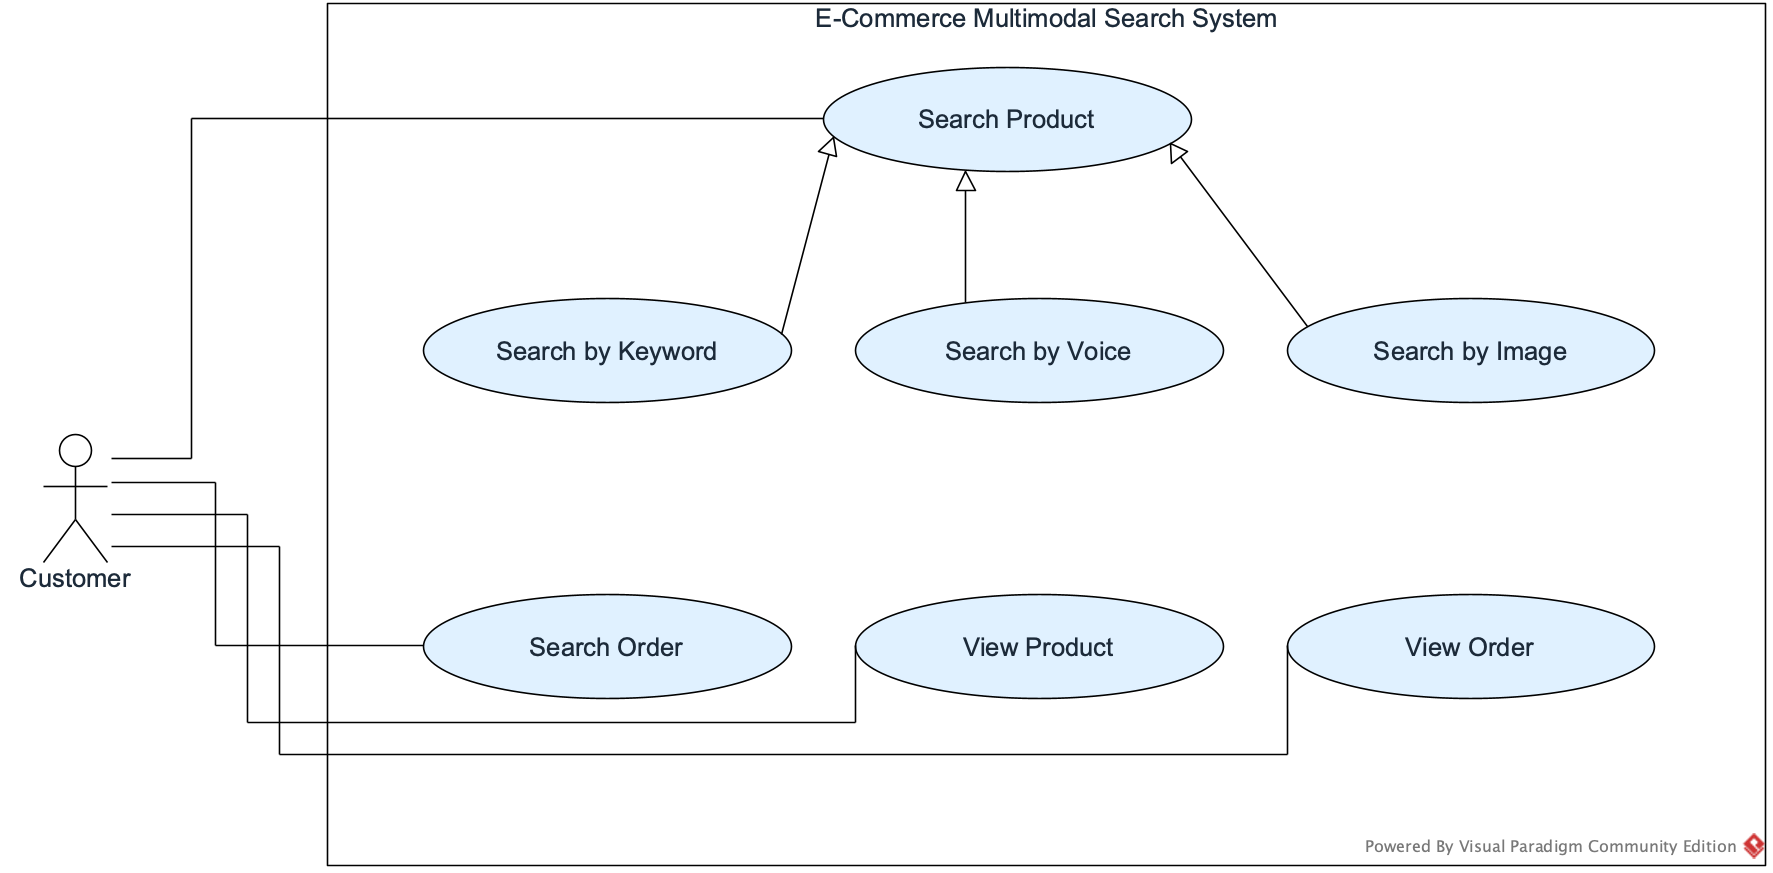
\includegraphics[width=0.88\linewidth]{../diagrams/01_use_case.png}
\caption{Use-case diagram created in Visual Paradigm.}
\end{figure}

The diagram has one Customer actor and all seven use cases required by the assignment. Search by Keyword, Search by Voice, and Search by Image specialize Search Product. Search Order, View Product, and View Order are separate customer goals. The actor is outside the system boundary; each use case is inside it.

\begin{table}[H]\small
\caption{Main use-case flows}
\begin{tabularx}{\linewidth}{@{}p{34mm}Y@{}}\toprule
Use case & Main flow and result \\ \midrule
Search Product & Customer submits text, a transcript, or an image. The system builds a query, retrieves and ranks products, then displays the top results. \\
Search Order & Customer supplies an order ID or asks for the latest order. The system checks ownership and returns the status, or reports no match. \\
View Product & Customer selects a product ID. The system returns its record or reports that it is unavailable. \\
View Order & Customer selects an order found under the same customer ID and sees its details. \\
\bottomrule\end{tabularx}
\end{table}

\clearpage
\begin{landscape}
\section{Three-layer architecture}
\thispagestyle{empty}
\begin{figure}[H]\centering
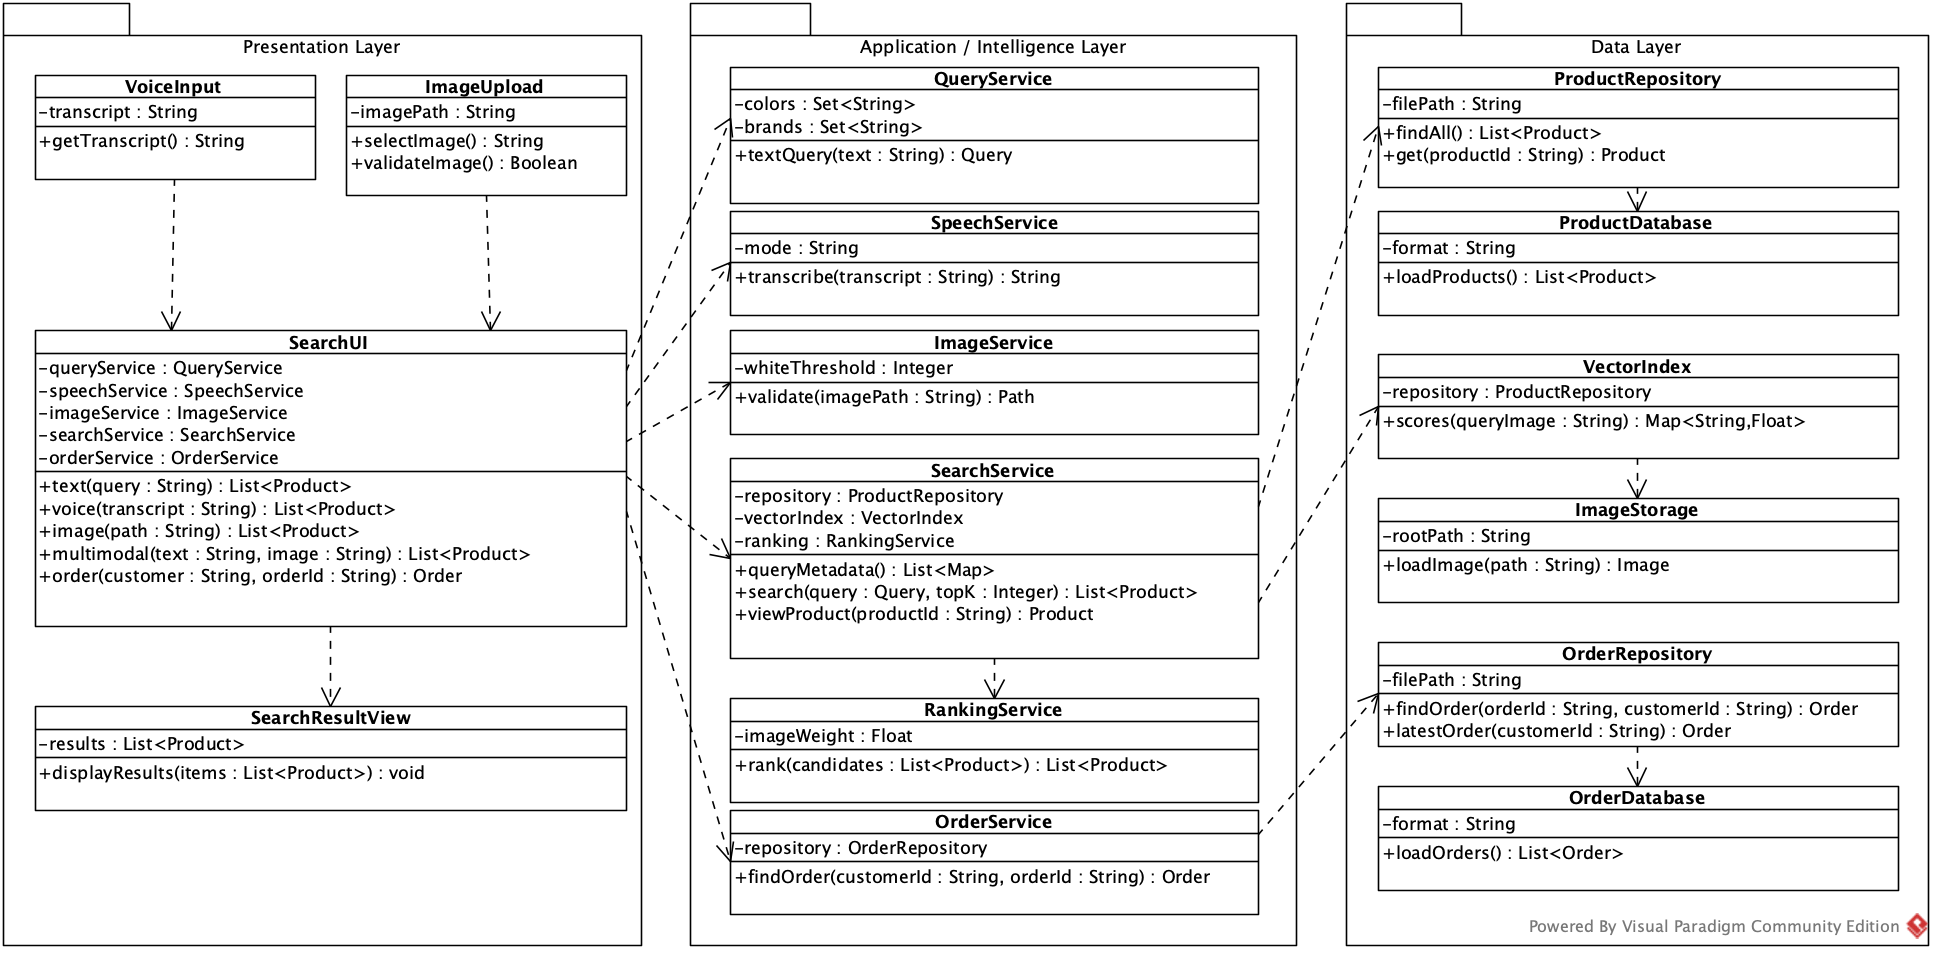
\includegraphics[width=0.96\linewidth]{../diagrams/02_three_layer_architecture.png}
\caption{Three-layer class diagram with native Visual Paradigm classes and UML dependencies.}
\end{figure}

\small
\textbf{Presentation} collects input and displays results. \textbf{Application / Intelligence} prepares queries, performs search and ranking, and handles orders. \textbf{Data} provides repositories, JSON records, product images, and the Vision image index. Dashed dependency arrows point from the class that uses a service to the class it uses. The main flow is SearchUI $\rightarrow$ application services $\rightarrow$ data services. Each class uses Visual Paradigm's default name, attributes, and operations compartments.
\end{landscape}

\clearpage
\begin{landscape}
\section{Voice-search sequence}
\thispagestyle{empty}
\begin{figure}[H]\centering
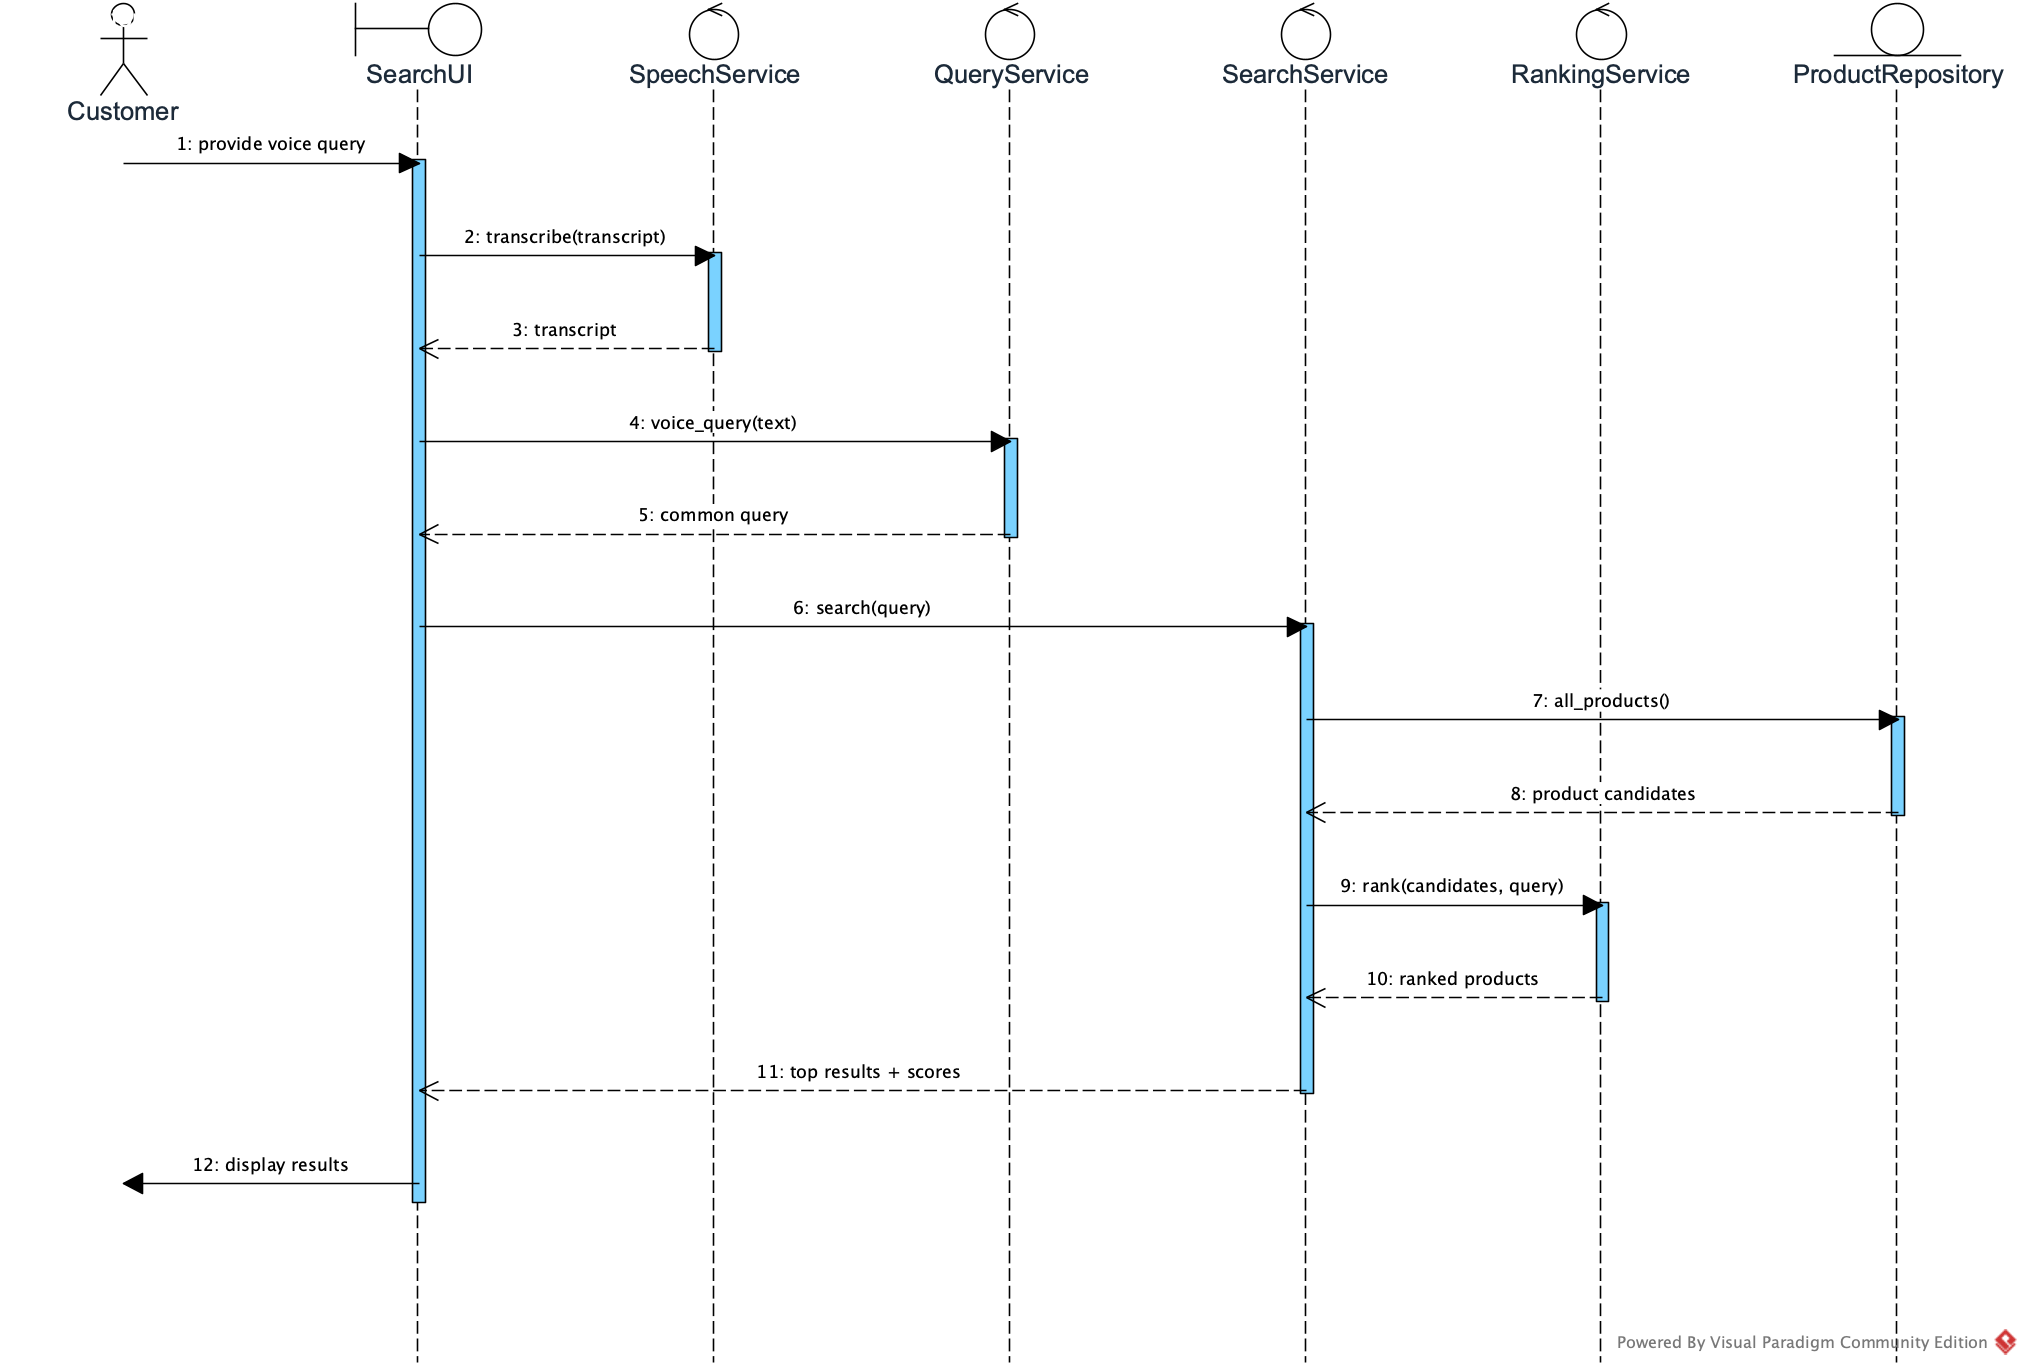
\includegraphics[width=0.70\linewidth]{../diagrams/03_sequence_voice.png}
\caption{Voice-search sequence diagram. Boundary, control, and data-access roles are identified in the lifeline heads.}
\end{figure}
\small
\textbf{Main flow:}
\begin{enumerate}[leftmargin=1.5em,itemsep=1pt,topsep=2pt]
\item Customer provides voice input; browser speech recognition produces a transcript for SearchUI. The console version supplies that transcript directly.
\item SpeechService passes the text to QueryService, which creates a common query.
\item SearchService retrieves candidates from ProductRepository, ranks them, and returns results for SearchUI to display.
\end{enumerate}
\end{landscape}

\nextsection{Data and implementation}
The teaching catalog has 12 synthetic products and three sample orders. This is more than the assignment's ten-product minimum. It supports short text, voice-transcript, and order examples; its generated product pictures were removed. The browser's text, voice-transcript, image, and combined search instead use 500 real Open Food Facts products and photos.

\begin{table}[H]\small
\caption{Data records used by the prototype}
\begin{tabularx}{\linewidth}{@{}p{29mm}Y Y@{}}\toprule
Record & Main fields & Storage \\ \midrule
Product & ID, name, category, color, price, stock, image & \path{data/products.json}; real photos in \path{data/openfoodfacts/images/} \\
Order & ID, customer ID, date, status, total & \path{data/orders.json} \\
Order item & Product ID, quantity, unit price & Nested in an order record \\
Image feature print & Product photo and Vision image features & Indexed in memory by the local Swift process \\
\bottomrule\end{tabularx}
\end{table}

\begin{figure}[H]\centering
\begin{tabular}{@{}p{29mm}cc@{}}
 & \small Query photo & \small Indexed front photo \\
\small Pasta sauce & \includegraphics[width=.32\textwidth,height=59mm,keepaspectratio]{../data/openfoodfacts/images/5010251561958_query.jpg} &
\includegraphics[width=.32\textwidth,height=59mm,keepaspectratio]{../data/openfoodfacts/images/5010251561958_front.jpg} \\[3mm]
\small Noodles & \includegraphics[width=.32\textwidth,height=59mm,keepaspectratio]{../data/openfoodfacts/images/01758979_query.jpg} &
\includegraphics[width=.32\textwidth,height=59mm,keepaspectratio]{../data/openfoodfacts/images/01758979_front.jpg}
\end{tabular}
\caption{Real Open Food Facts query and gallery photos (CC BY-SA 3.0). The sauce is retrieved first; the noodles front photo is outside the top five.}
\end{figure}

\clearpage
\pagestyle{fancy}
\thispagestyle{fancy}
\subsection*{Service responsibilities and search logic}
\begin{table}[H]\small
\caption{UML classes and Python modules}
\begin{tabularx}{\linewidth}{@{}p{34mm}Y@{}}\toprule
Layer / component & Implementation \\ \midrule
Presentation & SearchUI collects mode-specific input and displays results. \\
Query handling & QueryService normalizes input into a common query. \\
Voice and image & SpeechService passes the transcript; ImageService validates the uploaded photo. \\
Product search & SearchService retrieves candidates; RankingService sorts them. \\
Order search & OrderService handles order ID and latest-order requests. \\
Data & Repositories load JSON; VectorIndex compares Vision features and returns package text. \\
\bottomrule\end{tabularx}
\end{table}

\textbf{Text and voice.} QueryService lowercases text, normalizes a small set of category synonyms, and detects common colors, brands, and price limits. SearchService applies the detected filters before ranking. In the browser, the Web Speech API turns microphone speech into editable text. SearchUI then sends that transcript through SpeechService and the same query path. The console example and saved voice checks use supplied transcripts, so they do not measure recognition accuracy.

\textbf{Image search.} ImageService validates the uploaded file. VectorIndex uses Apple's \href{https://developer.apple.com/documentation/vision/vngenerateimagefeatureprintrequest}{Vision feature-print API} to describe each catalog photo and the query photo. Vision measures their visual distance $d$; a smaller distance means a closer match. Apple Vision's text recognizer also reads visible package text from the query. The application converts distance to similarity $S_i=1/(1+d)$ and compares recognized words with the product name and brand. Both services run locally on macOS through Swift.

\textbf{Ranking.} The business score $B$ combines popularity and in-stock status. Text or voice search uses $0.9S_t+0.1B$. For image search, $S_o=0.8C+0.2R$, where $C$ is the share of informative product-name words recognized in the photo and $R$ is 1 when a brand word is recognized, or 0 otherwise. V02 uses $0.9S_i+0.1S_o$; this retains visual similarity as the main signal and uses package text to resolve close candidates. Text-image search uses $0.4S_t+0.4S_i+0.1S_o+0.1B$. Retrieval selects eligible candidates; RankingService sorts those candidates by score.

\textbf{External data.} The browser and evaluation use 500 real grocery products and 100 separate alternate-view query images from Open Food Facts. Gallery and query photos are kept as distinct files; a query photo is never used in the gallery index. Every product has a barcode and title; 350 have a brand and 204 have a usable broad category. Source selection, attribution, and license details are in \path{data/openfoodfacts/DATASET.md}.

\nextsection{Demonstration}
\begin{figure}[H]\centering
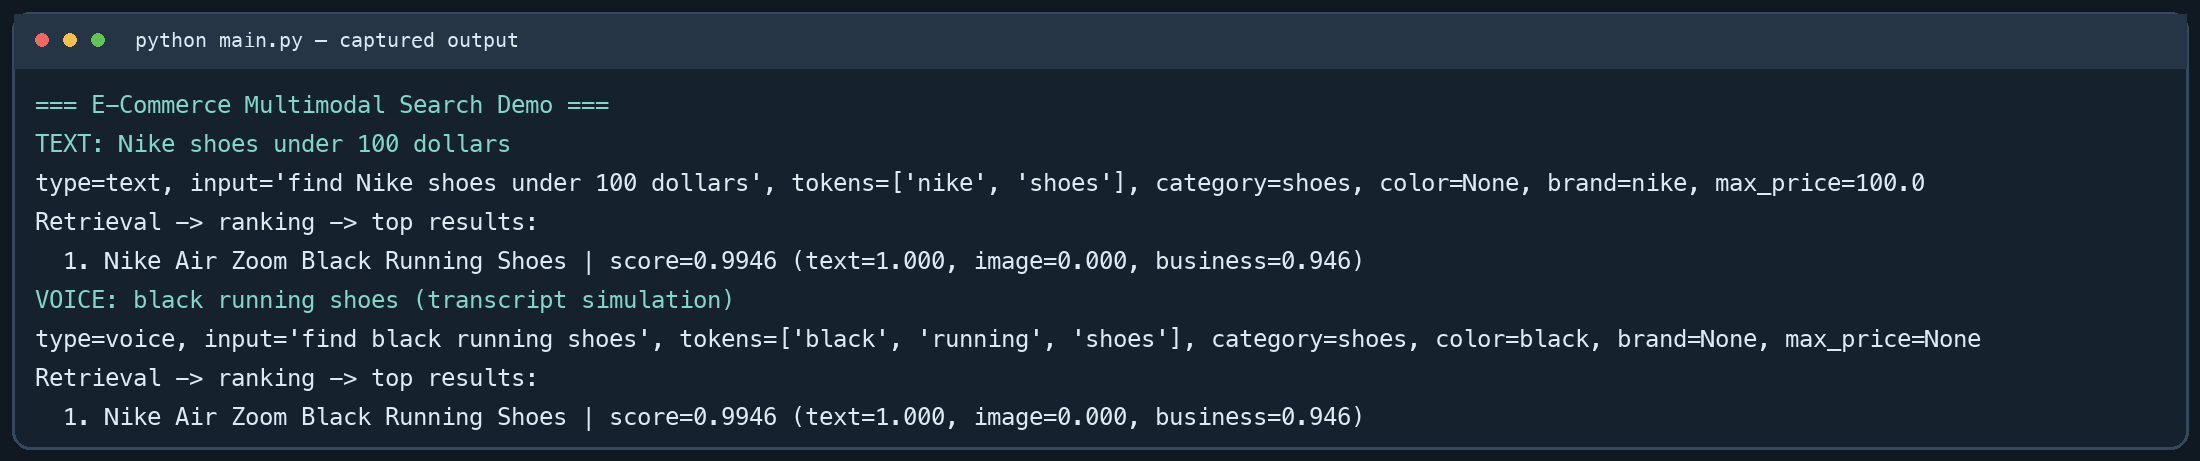
\includegraphics[width=0.90\linewidth]{../demo/console_capture.png}
\caption{Console text and simulated-voice demonstration generated by \code{python main.py}.}
\end{figure}

The console output shows the input, normalized query, ranked results, and scores for text and a supplied voice transcript. The order demo finds order \code{20261001} for customer \code{C001}; the same request returns no order for customer \code{C002}. In the browser, the Voice tab can capture speech from the microphone, show the recognized text, and run the same voice search.

\begin{figure}[H]\centering
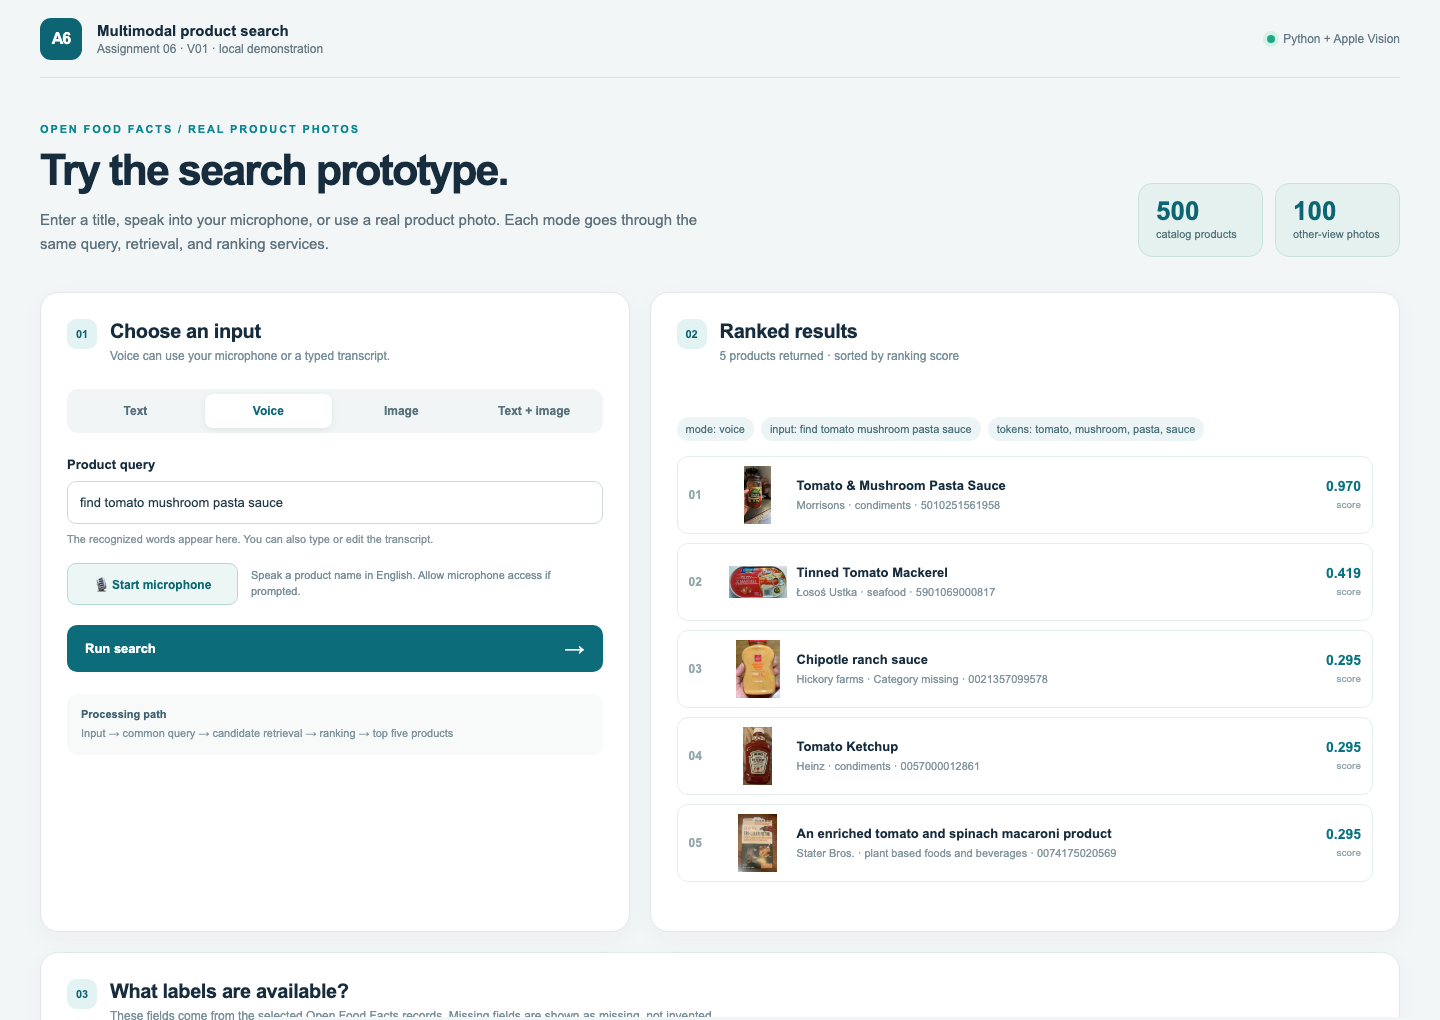
\includegraphics[width=0.78\linewidth]{../demo/voice_capture.png}
\caption{Browser Voice tab with microphone control and ranked results from an example transcript.}
\end{figure}

\begin{table}[H]\small
\caption{Labels visible in the browser's real-product catalog}
\begin{tabularx}{\linewidth}{@{}p{36mm}p{30mm}Y@{}}\toprule
Field & Availability & How it is used \\ \midrule
Barcode and name & 500/500 products & Product identity and title lookup. \\
Brand & 350/500 products & Display and keyword matching when present. \\
Broad category & 204/500 products & Display; 52/100 image queries have a usable category check. \\
Query's true barcode & 100/100 photos & Correct answer for exact-product image retrieval. \\
\bottomrule\end{tabularx}
\end{table}

Shop prices and inventory are absent from Open Food Facts; the real-photo image ranking does not use placeholder business fields. Generated teaching images are excluded from the evaluation.

\begin{figure}[H]\centering
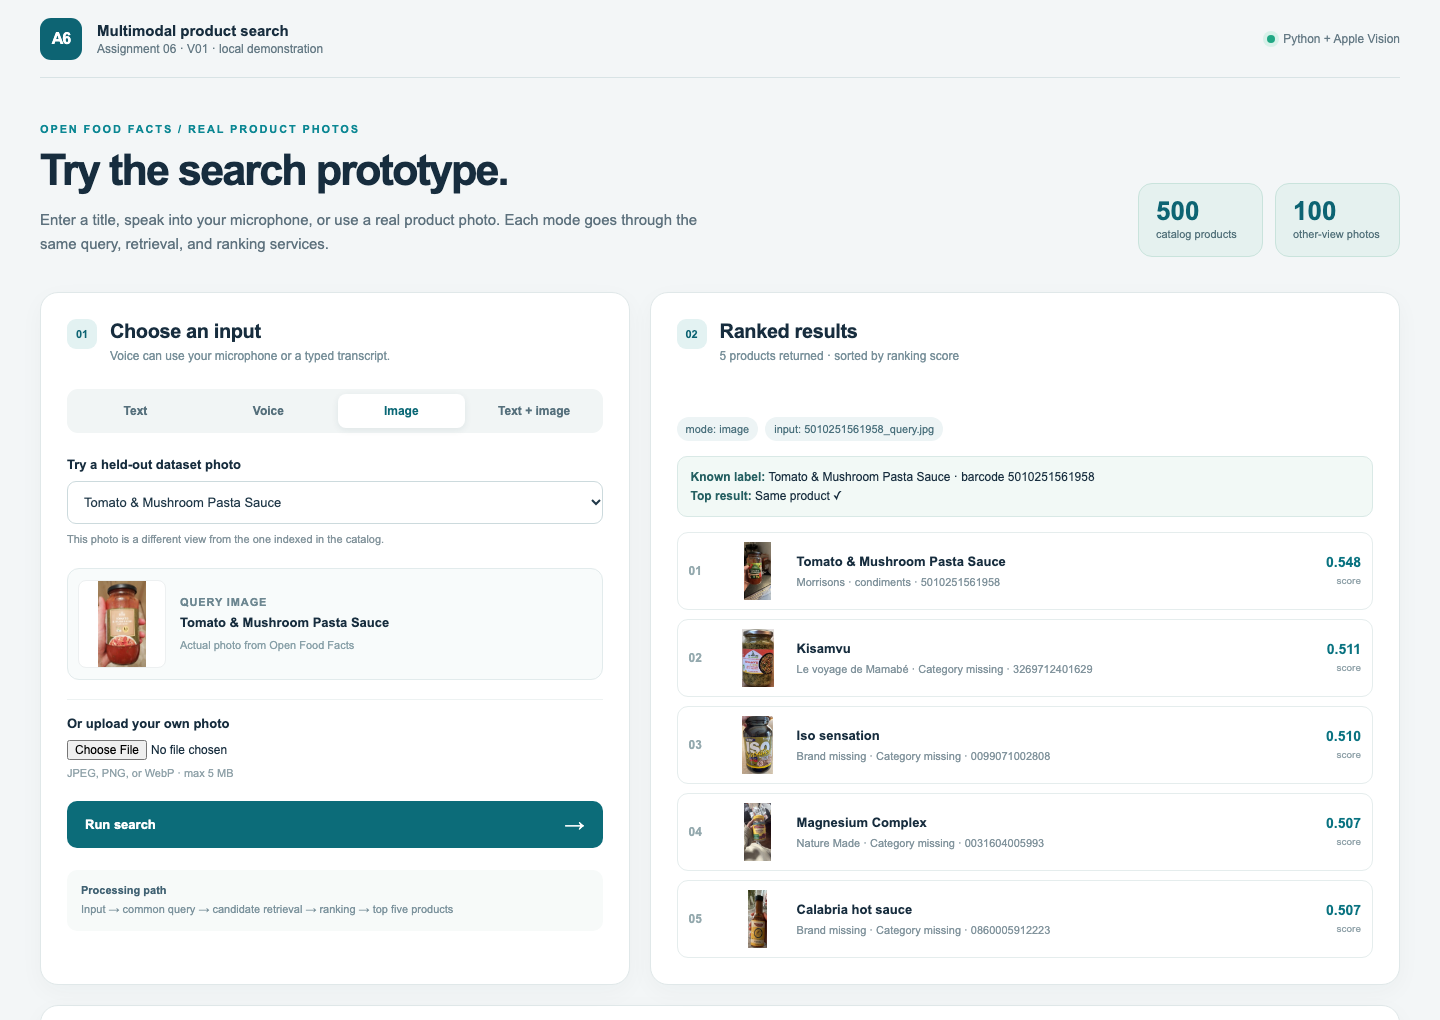
\includegraphics[width=0.85\linewidth]{../demo/web_capture.png}
\caption{Local Python web demonstration searching with a real Open Food Facts query photo. The known barcode and ranked products are shown.}
\end{figure}

\begin{table}[H]\small
\caption{Required search modes and one extension}
\begin{tabularx}{\linewidth}{@{}p{25mm}Y Y@{}}\toprule
Mode & Example input & First result \\ \midrule
Text & \code{find Nike shoes under 100 dollars} & Nike Air Zoom Black Running Shoes \\
Voice & \code{find black running shoes} (console transcript) & Nike Air Zoom Black Running Shoes \\
Image & Alternate photo of Tomato \& Mushroom Pasta Sauce & Tomato \& Mushroom Pasta Sauce \\
Text + image & \code{Tomato Mushroom Pasta Sauce} and the photo & Tomato \& Mushroom Pasta Sauce \\
\bottomrule\end{tabularx}
\end{table}

The browser runs from \code{web\_demo.py} at \code{127.0.0.1:8765}; it accepts a provided dataset photo or an uploaded photo. Its image result is a genuine Apple Vision result on the 500-product gallery. The first result is correct for the shown sauce query, while the full 100-photo evaluation below includes failures.

\nextsection{Evaluation}
\textbf{Question and data.} Does package text improve exact-product image retrieval? Product records come from the official Open Food Facts \href{https://static.openfoodfacts.org/exports/products.random-modulo-1000.tar.gz}{random-modulo-1000 sample}; photos come from its image store. The test uses 500 gallery products and 100 separate alternate-view query photos. Each gallery photo is the product's front view; the query photo is kept out of the index. A result is correct when its barcode matches the query label. Top-1 and top-5 are reported.

\textbf{Fair comparison.} The evaluation calls the same SearchUI, SearchService, and Apple Vision code as the browser. A fixed random seed separates 20 photos for weight selection and 80 held-out photos for the final comparison. On the 20 calibration photos, it tries package-text weights from 0.0 to 0.8 in steps of 0.1. It selects the weight with the best top-1 result, then top-5; ties prefer the smaller weight. The chosen weight is 0.1. The held-out labels do not guide weight selection. V01 and V02 are compared on the exact same 80 test photos.

\begin{table}[H]\small
\caption{Exact-product image retrieval on the held-out photos}
\begin{tabularx}{\linewidth}{@{}p{42mm}p{40mm}p{35mm}Y@{}}\toprule
Method & Top-1 correct & Top-5 correct & Plain-language result \\ \midrule
V01 Apple Vision features & 20/80 (25\%) & 23/80 (28.8\%) & Visual similarity only. \\
V02 Vision + package text & 28/80 (35\%) & 32/80 (40\%) & 8 more first-place matches and 9 more top-five matches. \\
Change & +8 queries (+10 pp) & +9 queries (+11.2 pp) & pp means percentage points; no V01 top-1 match was lost. \\
\bottomrule\end{tabularx}
\end{table}

The 20 calibration photos yielded 3/20 top-1 and 4/20 top-5 matches at the selected weight. On the held-out set, package text corrected cases such as \emph{White Corn Chips} and \emph{Apple Juice}; eight V01 misses became top-1 matches. This result is encouraging but still leaves 52 of 80 exact products outside first place. The sample is grocery-focused and does not establish performance on other stores or product types. Per-query results, the weight sweep, and the split details are in \path{demo/v02_openfoodfacts_evaluation.json}. The earlier all-100 V01 score is retained in \path{demo/openfoodfacts_evaluation.json} for reference and is not used as the paired comparison.

The supporting functional checks on the teaching catalog remain 16/16 expected text and voice matches, 3/3 handled no-match queries, and 4/4 order-access checks. Supplied voice transcripts test retrieval after transcription; live microphone recognition is demonstrated but its accuracy is not measured.

\nextsection{Discussion and conclusion}
The prototype meets the required tasks: it defines the customer requirements, models all required use cases and the three layers in Visual Paradigm, illustrates voice search, and implements text, voice-transcript, image, and ranked results in Python. V02 adds package OCR to image ranking and improves held-out exact-product retrieval from 20/80 to 28/80 at top-1. The browser adds live microphone transcription and demonstrates text-image fusion, price filtering, and order ownership checks.

The main limitation is exact-product image retrieval: the V02 method still misses the first result for 52 of 80 held-out photos. OCR can fail on small, angled, or obscured packaging text, and the feature-print model also requires macOS and Swift. The teaching catalog is small; the real-photo sample is grocery-focused and much smaller than a real store. Microphone recognition depends on browser support, permission, and the browser's recognition service; its accuracy is not measured here. The supplied customer ID is not an authentication mechanism.

A practical next step is to evaluate the combined method on a broader, independently sourced product catalog and improve OCR handling for rotated or partially visible labels. The current service boundaries allow that work within the image index without moving search logic into the user interface.

\textbf{Reproducibility.} The GitHub repository contains the editable \code{.vpp} project, Python source, browser interface, teaching records, README, tests, and saved evaluation results. The prepared Open Food Facts photos and metadata are provided as a separate ZIP on Google Drive. The README provides a tested \code{gdown} command, checksum, and extraction steps. The UML project can be rebuilt with \path{tools/build_vp.py}; the report uses the supplied Assignment 06 handout as its specification.

\textbf{Submission links.} GitHub source and report: \href{https://github.com/scalliontor/A6_V01_VuHungAnh}{github.com/scalliontor/A6\_V01\_VuHungAnh}. Prepared dataset: \href{https://drive.google.com/drive/folders/1Ta9vMurnYoJzvNcP23Iflulr-EVWIx58?usp=sharing}{drive.google.com/drive/folders/1Ta9vMurnYoJzvNcP23Iflulr-EVWIx58}.

\textbf{Dataset attribution.} Product records are from Open Food Facts contributors. The database is under ODbL 1.0 and the Database Contents License; product images are under CC BY-SA 3.0. Selection and image resizing are documented in \path{data/openfoodfacts/DATASET.md} inside the Drive ZIP. This coursework is not endorsed by Open Food Facts. See the official \href{https://github.com/openfoodfacts/openfoodfacts-ai/blob/develop/data-sets.md}{dataset sample documentation} and \href{https://openfoodfacts.github.io/documentation/docs/Product-Opener/api/tutorials/license-be-on-the-legal-side/}{license guidance}.

\end{document}
